\documentclass{article}

\usepackage{iclr2026_conference,times}
\input{math_commands.tex}
\usepackage{hyperref}
\usepackage{url}
\usepackage{booktabs}
\usepackage{graphicx}
\usepackage{amsmath}
\usepackage{amssymb}
\usepackage{amsthm}

\newtheorem{proposition}{Proposition}

\title{Best-of-N Search Amplifies Option-Boundary Errors in Hierarchical Skill Planning}

\author{Anonymous Authors}

\begin{document}

\maketitle

\begin{abstract}
Hierarchical robot planners increasingly compose learned skills, options, or subgoals with a high-level scorer.
Best-of-N inference is an attractive way to improve such planners at test time: sample many abstract plans and execute the one with the highest proxy score.
This paper studies a failure mode that is specific to temporal abstraction.
When the proxy score is miscalibrated at option boundaries, increasing \(N\) can select plans that look better abstractly but are less executable because their initiation sets, termination distributions, and handoffs are unsafe.
We build a controlled option-chain simulator that exposes this mechanism, prove an exact finite-population law for true utility under max-proxy selection, and validate it numerically.
In the main sweep, raw Best-of-N raises the selected proxy score by \(7.52\) while reducing chain executability at \(N=512\) to \(15.2\%\) of its \(N=1\) value.
We propose Boundary-Calibrated Option Sieve, a repair that uses only public boundary evidence and improves large-\(N\) true utility by \(0.53\) in the controlled setting.
The result is not a benchmark robot claim; it is a mechanism study and a diagnostic target for real skill-chain planners.
\end{abstract}

\section{Introduction}

Robotic control systems often separate long-horizon reasoning from low-level execution by planning over temporally extended skills or options.
This separation is useful, but it also creates boundaries: an option can only be initiated on a subset of states, it terminates in a distribution rather than at a single abstract symbol, and its output state becomes the next option's input.

Best-of-N inference appears to be a nearly free improvement for this setting.
Given a high-level proxy scorer, one samples \(N\) candidate option plans and executes the plan with the largest score.
The intuition is that larger \(N\) should discover better abstract plans.
This intuition can fail when the proxy mistakes ambitious subgoals for feasible chains.
The failure is not simply that rewards are noisy.
It is that the selected plan increasingly lives in the tail where option boundaries are least calibrated.

We make three contributions.
First, we isolate the option-boundary version of Best-of-N overoptimization.
Second, we give an exact finite-population law that predicts selected true utility from proxy ranks.
Third, we introduce Boundary-Calibrated Option Sieve, a simple repair that downweights unsafe handoff evidence without accessing hidden true execution labels.

\section{Related Work}

The options framework formalizes temporal abstraction through initiation sets, intra-option policies, and termination conditions \citep{sutton1999between,precup2000temporal}.
Hierarchical RL methods such as MAXQ \citep{dietterich2000hierarchical}, surveys of HRL \citep{barto2003recent}, and option-critic \citep{bacon2017optioncritic} study how to learn or compose such abstractions.
Our focus is narrower: what happens when a high-level search procedure over learned options selects on a proxy that is miscalibrated at option boundaries.

Best-of-N sampling is a simple inference-time optimizer, and proxy overoptimization has been studied in reward-model settings \citep{gao2023scaling}.
This work borrows the selection-pressure lens but asks where the proxy error comes from in hierarchical robot skill planning.
The answer studied here is option-boundary feasibility: initiation support, stochastic termination, and handoff reachability.

\section{Option-Boundary Model}

We use a controlled option world rather than a benchmark suite so that the mechanism is observable.
Each option \(o\) has an initiation center \(c_o\), radius \(r_o\), stochastic termination mean \(m_o\), termination noise \(\sigma_o\), nominal reward \(R_o\), and reliable span \(d_o\).
Given an abstract state estimate \(x_t\), the option initiation probability decreases with the margin \(r_o - |x_t-c_o|\).
A long option can be attractive under nominal reward but unreliable if its span exceeds \(d_o\).
Termination drift propagates into the next handoff.

A plan \(\tau=(o_1,\ldots,o_H)\) has hidden true executability \(E(\tau)\), true utility \(U(\tau)\), proxy score \(S(\tau)\), and public diagnostics:
\[
D(\tau)=
\{\text{initiation violation},\ \text{termination drift},\ \text{reachability gap},\ \text{boundary surprise}\}.
\]
The miscalibrated proxy rewards nominal value and ambitious subgoal distance while under-penalizing or positively correlating with unsafe boundary evidence.

\section{Finite-N Selection Law}

\begin{proposition}
Let \(P=\{(S_i,U_i)\}_{i=1}^M\) be a finite proposal population with deterministic tie-breaking, sorted by increasing proxy score.
Draw \(N\) candidates independently and uniformly with replacement from \(P\), and select the candidate with maximum proxy score.
Then
\[
\mathbb{E}[U_{\mathrm{selected}}(N)]
=\sum_{r=1}^{M} U_{(r)}
\left[\left(\frac{r}{M}\right)^N-\left(\frac{r-1}{M}\right)^N\right].
\]
\end{proposition}

\begin{proof}
The item at rank \(r\) is selected exactly when all \(N\) draws have rank at most \(r\) and at least one draw has rank \(r\).
The probability of this event is \((r/M)^N-((r-1)/M)^N\).
Linearity of expectation gives the result.
\end{proof}

The proposition does not by itself prove degradation.
It shows how increasing \(N\) concentrates mass on the high-proxy tail.
Degradation follows when that tail has low true utility, which is precisely the option-boundary condition tested in the experiments.

\section{Boundary-Calibrated Option Sieve}

Boundary-Calibrated Option Sieve ranks candidates by
\[
S_{\mathrm{sieve}}(\tau)=S(\tau)-\lambda B(D(\tau)),
\]
where \(B\) is a public boundary-risk score combining initiation violation, termination drift, reachability gap, boundary surprise, and the estimated chain executability.
The method uses no hidden execution labels, no true utility, and no oracle feasibility.
It is intentionally simple: its role is to test whether boundary evidence is the right repair axis.

\section{Experiments}

We run four checks.
First, the finite-N law is compared with Monte Carlo selection.
Second, raw Best-of-N is swept over \(N\).
Third, the boundary sieve is evaluated on the same candidate sets.
Fourth, controls replace the miscalibrated scorer with calibrated, oracle, random, and anti-correlated scorers.
All claims are audited by \verb|python -m bonoptions.experiments.run_claim_audit|.

\begin{figure}[t]
\centering
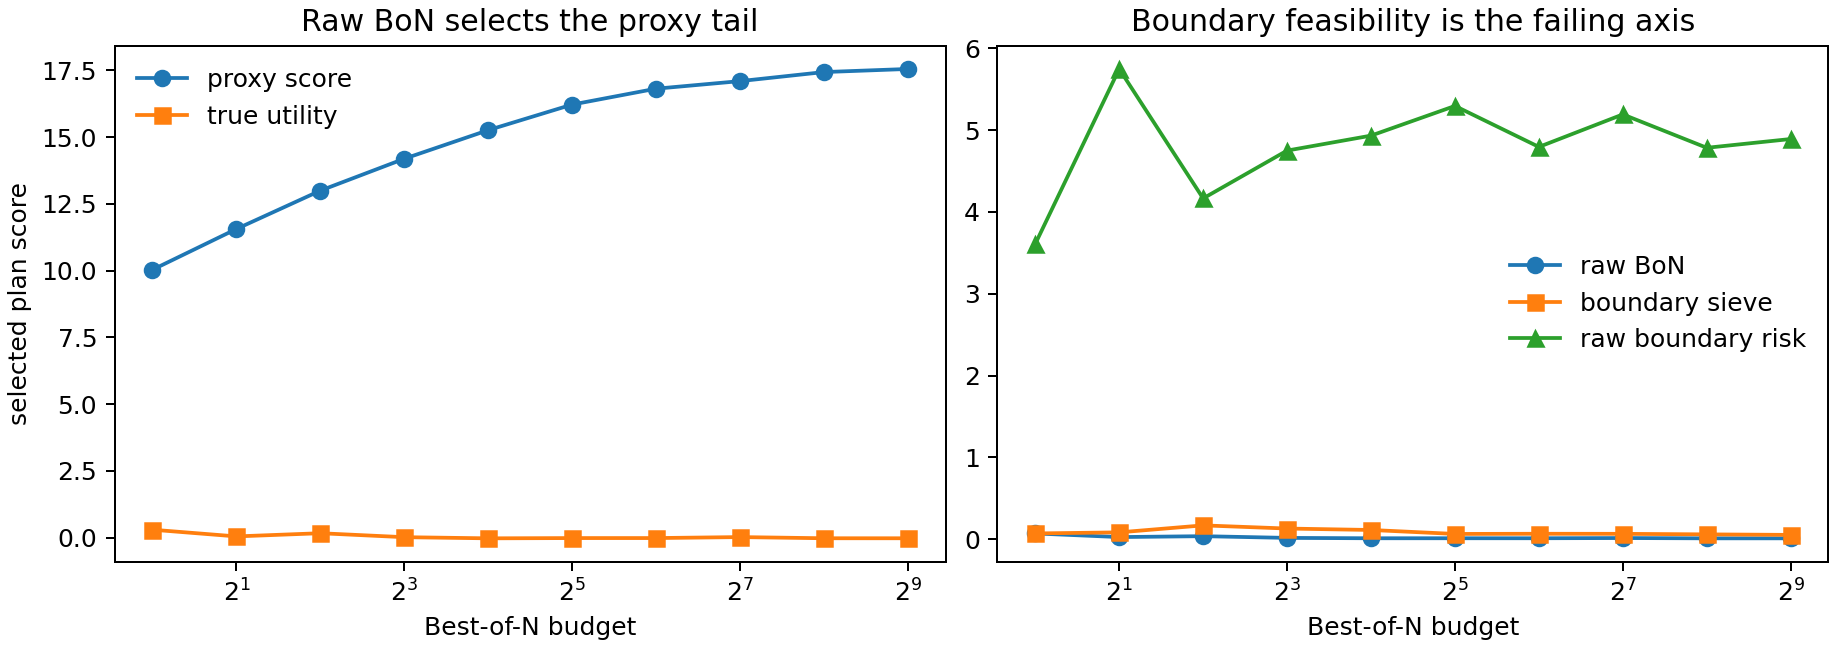
\includegraphics[width=\linewidth]{figures/bon_degradation.png}
\caption{Raw Best-of-N increases selected proxy score while moving toward less executable option chains. Boundary risk exposes the failing axis.}
\label{fig:degradation}
\end{figure}

\begin{figure}[t]
\centering
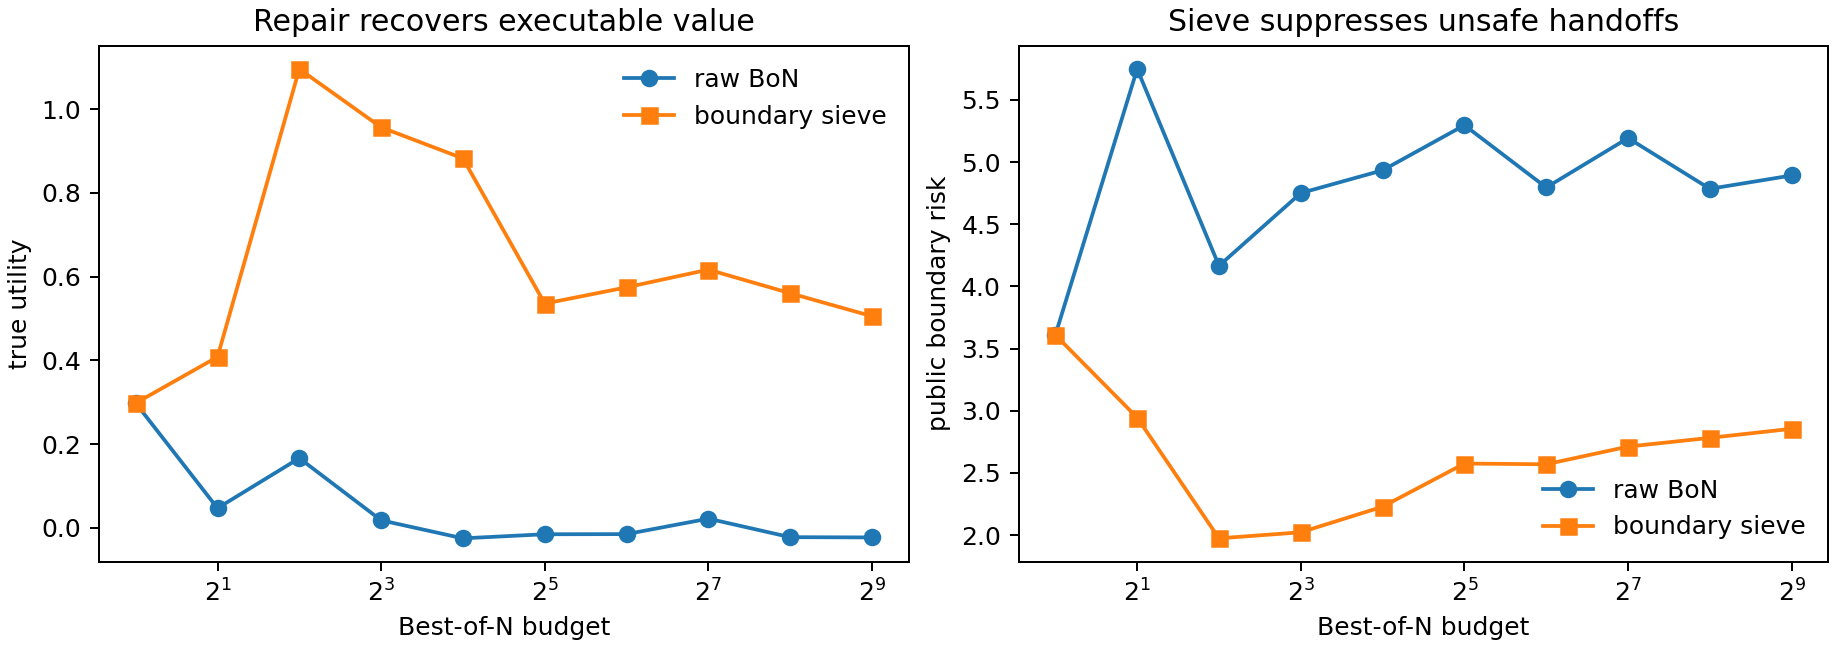
\includegraphics[width=\linewidth]{figures/repair_comparison.png}
\caption{Boundary-Calibrated Option Sieve selects lower-risk chains from the same candidate sets and recovers large-\(N\) true utility.}
\label{fig:repair}
\end{figure}

\begin{figure}[t]
\centering
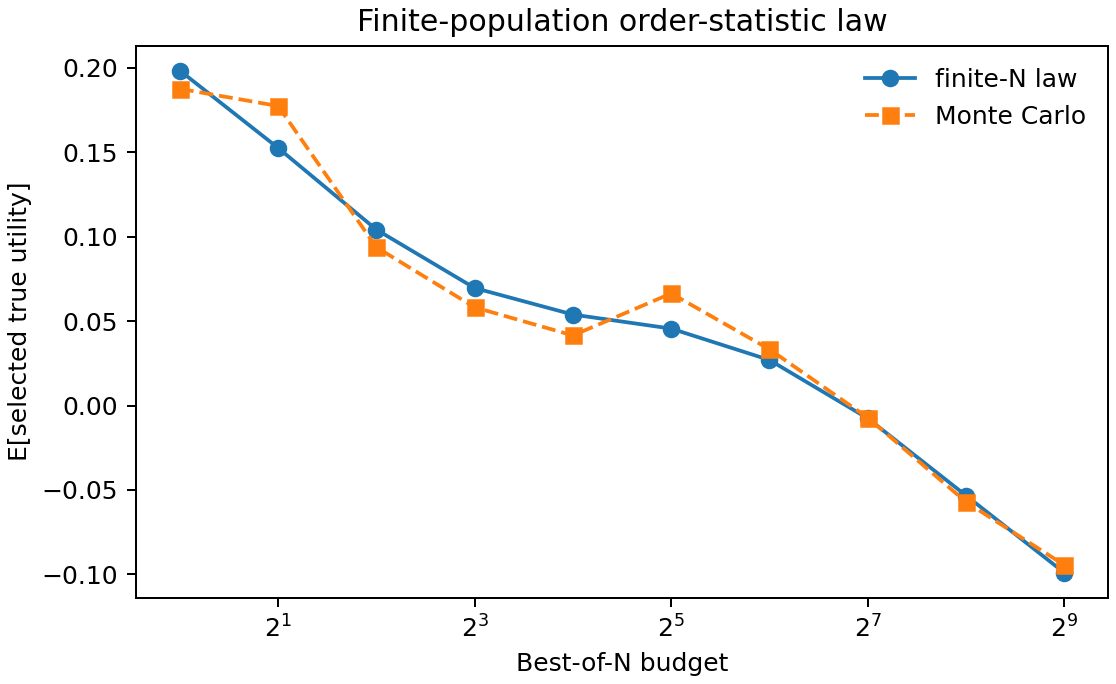
\includegraphics[width=0.72\linewidth]{figures/finite_n_law.png}
\caption{The exact finite-population law matches Monte Carlo selection. Current mean absolute error is \(0.0106\).}
\label{fig:finite}
\end{figure}

\paragraph{Main result.}
At \(N=512\), raw Best-of-N has a much higher proxy score than at \(N=1\), but its selected executability is only \(15.2\%\) of the \(N=1\) value.
True utility peaks at small \(N\) and then falls below zero under the miscalibrated proxy.
This supports the claim that proxy selection pressure can amplify option-boundary errors rather than merely improving abstract plans.

\paragraph{Repair.}
Using the same candidates, Boundary-Calibrated Option Sieve improves large-\(N\) true utility by \(0.53\) and improves executability.
The repair also reduces the selected public boundary-risk score.

\paragraph{Controls.}
The oracle feasibility scorer does not show the same failure and improves with \(N\).
The calibrated scorer is substantially more stable than the miscalibrated scorer.
Random and anti-correlated scorers behave as negative controls.
These controls suggest that the failure is not caused by candidate-set size alone.

\section{Limitations}

The study is controlled and low-dimensional.
The option diagnostics are hand-designed, and the repair is not claimed to be a final robot algorithm.
The results should not be read as benchmark evidence that one hierarchical planner outperforms another.
They show a mechanism that real systems should measure: whether high-level test-time search is selecting plans from the unsafe option-boundary tail.

\section{Conclusion}

Best-of-N inference is powerful but can be unsafe for hierarchical skill planners when proxy scores are miscalibrated at option boundaries.
The finite-N law explains the selection pressure, the simulator exposes the boundary mechanism, and Boundary-Calibrated Option Sieve demonstrates that public handoff diagnostics can repair much of the large-\(N\) degradation.
The next step is to learn these diagnostics from robot skill data and evaluate them on benchmark long-horizon manipulation tasks.

\bibliography{references}
\bibliographystyle{iclr2026_conference}

\appendix

\section{Reproducibility}

The public commands are:
\begin{verbatim}
python -m bonoptions.experiments.run_smoke
python -m bonoptions.experiments.run_all
python -m bonoptions.experiments.run_claim_audit
pytest
\end{verbatim}

The claim audit writes \verb|docs/claims.md| and \verb|results/claim_audit.json|.

\section{Claim Boundary}

The paper claims an option-boundary mechanism in a controlled simulator.
It does not claim real-robot benchmark superiority, universal degradation for all Best-of-N planners, or that the proposed sieve is optimal.

\end{document}
